%
% einleitung.tex -- Beispiel-File für die Einleitung
%
% (c) 2020 Prof Dr Andreas Müller, Hochschule Rapperswil
%
% !TEX root = ../../buch.tex
% !TEX encoding = UTF-8
%
\subsection{Kartesisch\label{geodaeten:section:Standardverfahren:Kartesisch}}

Für den kartesischen Raum mit dem metrischen Tensor
\begin{equation}
g_{i\!j} = \begin{pmatrix} 
	1 & 0 \\ 
	0 & 1 
\end{pmatrix},
\end{equation}
wollen wir die Christoffel-Symbole \eqref{geodaeten:equation:StandardverfahrenGeodaeten:ChristopherSymbole} berechnen.

Da der metrische Tensor $g_{i\!j}$ konstant ist und keine direkte Abhängigkeit von den Koordinaten aufweist, verschwinden alle Ableitungen.
Ohne weitere Berechnungen kann man also schliessen, dass
\begin{equation}
\frac{\partial g_{i\!j}}{\partial u^k} = 0 .
\end{equation}
Somit ergeben sich alle Christoffel-Symbole zu
\begin{equation}
\Gamma^i_{jk} = 0 .
\end{equation}

Denkt man an die Definition aus Abschnitt \ref{geodaeten:section:Standardverfahren}, macht dies durchaus Sinn.
Denn der Kartesische Raum ist nicht gekrümmt, weshalb keine Korrektur der Geraden notwendig ist.

Setzt man die Christoffel-Symbole in die allgemeine Geodätengleichung \eqref{geodaeten:equation:StandardverfahrenGeodaeten:Geodaetengleichung} ein, erhält man mit $u^1 = x(t)$
\begin{equation}
	\begin{alignedat}{3}
		&\ddot{u}^1 + \Gamma_{i\!j}^1 \dot{u}^i \dot{u}^j &\quad = \quad& 0 \\
		% &\ddot{u}^1 + 0_{i\!j} \cdot \dot{u}^i \dot{u}^j &\quad = \quad& 0\\
		%&\ddot{u}^1  &\quad = \quad& 0 \\
		&\ddot{x}(t) &\quad = \quad& 0
	\end{alignedat}
	\label{geodaeten:equation:Standardverfahren:Kartesisch:x}
\end{equation}
und mit $u^2 = y(t)$
\begin{equation}
	\begin{alignedat}{3}
		&\ddot{u}^2 + \Gamma_{i\!j}^2 \dot{u}^i \dot{u}^j &\quad = \quad& 0 \\
		% &\ddot{u}^2 + 0_{i\!j} \cdot \dot{u}^i \dot{u}^j &\quad = \quad& 0 \\
		% &\ddot{u}^2  &\quad = \quad& 0 \\
		&\ddot{y}(t) &\quad = \quad& 0  .
	\end{alignedat}
	\label{geodaeten:equation:Standardverfahren:Kartesisch:y}
\end{equation}

Da die zweite Ableitung in beiden Dimensionen Null ist, erkennt man bereits, dass es sich beim kürzesten Weg um eine Gerade handeln muss, was aus Erfahrung durchaus sinnvoll erscheint.

Setzt man nun zwei Punkte als Start und Endpunkt, kann man durch diese Nebenbedingungen eine konkrete Lösung erhalten.
Als Beispiel möchten wir den kürzesten Weg zwischen den Punkten $P_A = (1,1)$ und $P_B = (3,5)$ berechnen. 
Durch doppeltes Integrieren der Gleichung \eqref{geodaeten:equation:Standardverfahren:Kartesisch:x} erhält man
\begin{equation}
	\frac{d^2x}{dt^2} = 0 
	\Rightarrow \frac{dx}{dt} = c_1 
	\Rightarrow x(t) = c_1 \cdot t + c_2  .
	\label{geodaeten:equation:Standardverfahren:Kartesisch:equation1}
\end{equation}
Dabei sind $c_1$  und $c_2$ Integrationskonstanten. 

Wir sehen, die Gleichung entspricht einer parametrierten Geradengleichung mit $c_2$ als Startwert für $x(0)$ und $c_1$ als Steigung von $x(t)$. 
Mit $P_A(x_1,y_1)$ und $P_B(x_2,y_2)$ haben diese Gleichungen die Form
\begin{align}
	x(t) &= (x_2 - x_1) \cdot t + x_1 \\
	y(t) &= (y_2 - y_1) \cdot t + y_1 .
\end{align}
Da die Gerade durch den Startpunkt gehen muss ist der Startwert bei $t=0$ gegeben durch
\begin{equation}
	0 \cdot c_1 + c_2 = 1 \Rightarrow c_2 = 1 .	
\end{equation}
Die Steigung $c_1$ kann mithilfe von Endpunkt und Startpunkt berechnet werden als
\begin{equation}
	c_1 = x_2 - x_1 \\ = 3-1 \\ = 2
\end{equation}
und damit ist die Lösung der Geodätengleichung in $x$ gleich
\begin{equation}
	x(t) = 2t + 1 .
	\label{geodaeten:equation:StaKartesisch:LoesungX}
\end{equation}

Analog für $y(t)$ ergibt sich die Lösung der Geodätengleichung in $y$ zu
\begin{equation}
	y(t) = 4t + 1 .
	\label{geodaeten:equation:StaKartesisch:LoesungY}
\end{equation}
Die resultierende Kurve ist in Abbildung
\ref{geodaeten:figure:Standardverfahren:Kartesisch:figure1} dargestellt.
\begin{figure}
	\centering
	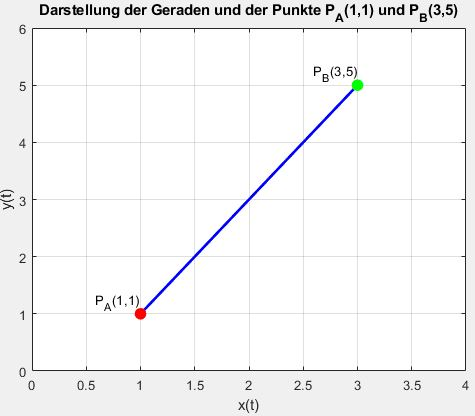
\includegraphics[width=10cm]{papers/geodaeten/Abbildungen/Standardverfahren/Kartesisch}
	\label{geodaeten:figure:Standardverfahren:Kartesisch:figure1}
	\caption{Darstellung der Kurve von x(t) und y(t) mit $t \in [0 , 1]$ Wie man sieht ist der kürzeste Weg von Punkt A zu Punkt B eine gerade.}
\end{figure}
